\documentclass[11pt,a4paper]{article}

\usepackage[margin=2.4cm]{geometry}
\usepackage{amsmath}
\usepackage{amssymb}
\usepackage{booktabs}
\usepackage{graphicx}
\usepackage{tikz}
\usepackage{xcolor}
\usepackage{enumitem}
\usepackage{pifont}
\usepackage[colorlinks=true,linkcolor=blue!50!black,urlcolor=blue!50!black]{hyperref}
\usetikzlibrary{shapes.geometric, arrows.meta, positioning, fit, backgrounds, calc}

\definecolor{cGreen}   {HTML}{D5E8D4}
\definecolor{cBlue}    {HTML}{DAE8FC}
\definecolor{cYellow}  {HTML}{FFF2CC}
\definecolor{cPurple}  {HTML}{E1D5E7}
\definecolor{cOrange}  {HTML}{FFE6CC}
\definecolor{cGray}    {HTML}{F0F0F0}
\definecolor{cRed}     {HTML}{F8CECC}
\definecolor{cDkGreen} {HTML}{82B366}
\definecolor{cDkBlue}  {HTML}{6C8EBF}
\definecolor{cDkYellow}{HTML}{D6B656}
\definecolor{cDkPurple}{HTML}{9673A6}
\definecolor{cDkOrange}{HTML}{D79B00}
\definecolor{cDkRed}   {HTML}{B85450}
\definecolor{cDkGray}  {HTML}{555555}

\tikzset{
  box/.style   ={rectangle, rounded corners=2pt, draw=cDkGray, fill=cGray,
                 align=center, font=\scriptsize, inner sep=4pt, minimum height=7mm},
  data/.style  ={box, fill=cBlue,   draw=cDkBlue},
  armA/.style  ={box, fill=cGreen,  draw=cDkGreen},
  armB/.style  ={box, fill=cYellow, draw=cDkYellow},
  armC/.style  ={box, fill=cOrange, draw=cDkOrange},
  stat/.style  ={box, fill=cPurple, draw=cDkPurple},
  ctrl/.style  ={box, fill=cRed,    draw=cDkRed},
  verdict/.style   ={box, fill=white,   draw=cDkGray, font=\scriptsize},
  ar/.style    ={-{Stealth[length=2mm]}, draw=cDkGray, thick},
  arf/.style   ={-{Stealth[length=2mm]}, draw=cDkGray, thick, dashed},
}

\newcommand{\dcor}{\operatorname{dCor}}
\newcommand{\Cov}{\operatorname{Cov}}
\newcommand{\Var}{\operatorname{Var}}
\newcommand{\E}{\mathbb{E}}
\newcommand{\R}{\mathbb{R}}

\title{\S27 --- Can TerraMind embeddings resolve sub-kilometre\\soil-moisture contrast?\\[2mm]
\large Design document, written before any code exists, for critique}
\author{Soil moisture project}
\date{2026-08-12}

\sloppy
\begin{document}
\maketitle

\begin{abstract}
\noindent
Six TxSON stations inside one 2.24\,km tile have observed mean soil moisture spanning
0.137--0.287\,m$^3$/m$^3$. The model predicts them at 19\,\% of that spread, with the
station ordering \emph{anti}-correlated with truth. This document specifies an experiment
that asks one question --- do the frozen TerraMind token embeddings contain information
that separates two stations a few hundred metres apart? --- and derives the mathematics
that makes the answer identifiable. Nothing here has been run. The purpose is to be
criticised before compute is spent.
\end{abstract}

\tableofcontents
\bigskip\hrule

\section{The observation}

\subsection{What the tile figure shows}

Figure~\ref{fig:tile} is \verb|figures/tile_context/ISMN_TxSON_CR200-18.pdf|. Six TxSON
stations fall inside one 224$\times$224 @ 10\,m tile (2.24\,km), separated by at most
936\,m. The tile is not uniform: 45\,m of relief, six land-cover classes, one station
(CR200-6) in crops in a valley bottom, the rest rangeland on slopes.

\begin{itemize}[nosep]
  \item \textbf{Observed} across-station spread $0.0601$\,m$^3$/m$^3$; level range $0.171$.
  \item \textbf{Predicted} across-station spread $0.0113 = 19\,\%$ of observed.
  \item $r(\text{predicted level},\ \text{observed level}) = -0.175$.
\end{itemize}

The same collapse holds on every dense tile: CR200-3 19\,\%, CR200-26 19\,\%,
CR1000-2 15\,\% --- all below the $0.35$ threshold at which
\verb|plot_network_timeseries.py| declares ``the map repeats $\sim$one series over the
whole tile''.

\subsection{Two facts that rule out the easy explanations}

\paragraph{It is not a readout artefact.} One might object that reading six stations off
\emph{one} tile's map is out-of-distribution, since only pixel $(112,112)$ is ever
supervised (\verb|model.py:779|). But reading each station from its \textbf{own} centred
patch --- exactly the training configuration --- still collapses: over the 18 OOS TxSON
stations, $\mathrm{sd}_{\text{pred}} = 0.0158$ against
$\mathrm{sd}_{\text{obs}} = 0.0633$, with $r = -0.11$.

\paragraph{It is not a general failure of level prediction.} Skill degrades monotonically
with separation and is perfectly healthy at continental range
(Table~\ref{tab:scale}, depth 0--10, station-mean level, from
\verb|eval_output/predictions_oos.parquet|).

\begin{table}[h]
\centering
\small
\begin{tabular}{lrrrrr}
\toprule
scale & $n$ & $\mathrm{sd}_{\text{obs}}$ & $\mathrm{sd}_{\text{pred}}$ & ratio & $r$ \\
\midrule
between networks   & 21 & 0.0578 & 0.0525 & 0.91 & $+0.85$ \\
within USCRN       & 12 & 0.0967 & 0.0851 & 0.88 & $+0.89$ \\
within SCAN        & 33 & 0.1029 & 0.0868 & 0.84 & $+0.78$ \\
within SNOTEL      & 73 & 0.0715 & 0.0442 & 0.62 & $+0.31$ \\
within COSMOS-UK   &  6 & 0.0525 & 0.0356 & 0.68 & $-0.05$ \\
within TxSON       & 18 & 0.0633 & 0.0158 & \textbf{0.25} & $\mathbf{-0.11}$ \\
within one tile    &  6 & 0.0601 & 0.0113 & \textbf{0.19} & $\mathbf{-0.18}$ \\
\bottomrule
\end{tabular}
\caption{Level skill by spatial scale. The model resolves \emph{where is wetter} at
$\ge 10$\,km and not below.}
\label{tab:scale}
\end{table}

This is consistent with everything measured earlier: \S23 found the painted 224$^2$
structure \emph{anti}-correlated with the landscape ($r(\text{anomaly},\text{DEM}) =
-0.04$ to $+0.21$) with 64--83\,\% of variance on the 14$\times$14 token grid;
\S24.12 found site identity dominates the prediction and its share grows with depth;
\S22 found ``the model emits nearly the same spread at every station''.

\subsection{Why the inputs make this the expected outcome}

For the six CR200-18 stations, almost the entire input is shared:

\begin{itemize}[nosep]
  \item \textbf{ERA5-Land ($\sim$9\,km) is byte-identical} for all six
        (\verb|dataset.py:1045|) and supplies 365 of $\sim$600 sequence tokens ---
        numerically dominant in the FiLM context vector (\verb|model.py:743|).
        SIF ($\sim$5\,km) and TWSA (GRACE) likewise identical.
  \item \textbf{Soil is OpenLandMap 250\,m} resampled to 30\,m. The six stations differ by
        3\,\% clay, 4\,\% sand, 1 pH unit --- noise.
  \item \textbf{The finest satellite scale the model sees is 320\,m, not 160\,m.}
        \verb|dataset.py:212| gives \verb|widths = [1,3,5,7]| $\Rightarrow$
        2$\times$2 / 6$\times$6 / 10$\times$10 / 14$\times$14 token windows. The
        \verb|model.py:109| docstring claiming a 1$\times$1 centre scale is wrong.
        \verb|dataset.py:306| additionally drops 50\,\% of tokens \emph{before} pooling,
        which hits the 4-token finest scale hardest.
  \item \textbf{No terrain derivative exists anywhere} --- DEM enters only as a pooled
        TerraMind L12 embedding.
  \item \textbf{No station identity, no per-station bias, no per-station label
        normalisation}; \verb|dataset.py:1074-1081| emits raw m$^3$/m$^3$, and decoder
        \verb|BatchNorm2d| (\verb|model.py:176,179|) actively strips per-sample offsets.
\end{itemize}

A homogeneous prediction is therefore close to the Bayes-optimal answer \emph{given these
inputs}. The open question is whether better use of what we already hold could do better.

\begin{figure}[p]
\centering
\includegraphics[width=\textwidth]{../figures/tile_context/ISMN_TxSON_CR200-18.pdf}
\caption{\texttt{ISMN\_TxSON\_CR200-18} --- one 2.24\,km tile, six stations, 2019--2020.
Row 3 left: observed series, spread 0.0601. Row 3 right: predicted, spread 0.0113.
Row 4: observed vs predicted mean level, and the verdict box.}
\label{fig:tile}
\end{figure}

\clearpage
\section{The question}

\begin{quote}
Do the frozen TerraMind token embeddings contain information that distinguishes two
soil-moisture stations a few hundred metres apart --- and if so, at which layer, for
which modality, and does the model actually receive it?
\end{quote}

Scope is deliberately narrow. Terrain derivatives, 30\,m optics, higher-resolution soil,
multi-station supervision and any loss change are \emph{out of scope} and remain deferred.
No model, dataset or loss code is modified by this experiment.

\paragraph{One structural advantage of probing the representation rather than the model.}
The TerraMind encoder is \textbf{frozen} and was never trained on soil moisture. Therefore
train/val/test leakage does not apply to this experiment at all: a station in the training
split is no more ``seen'' by $\varphi$ than an out-of-sample one. Every colocated station
is usable regardless of split --- which matters, because colocated stations are scarce
(\S\ref{sec:inventory}).

\clearpage
\section{The experiment in one page}

\begin{figure}[h]
\centering
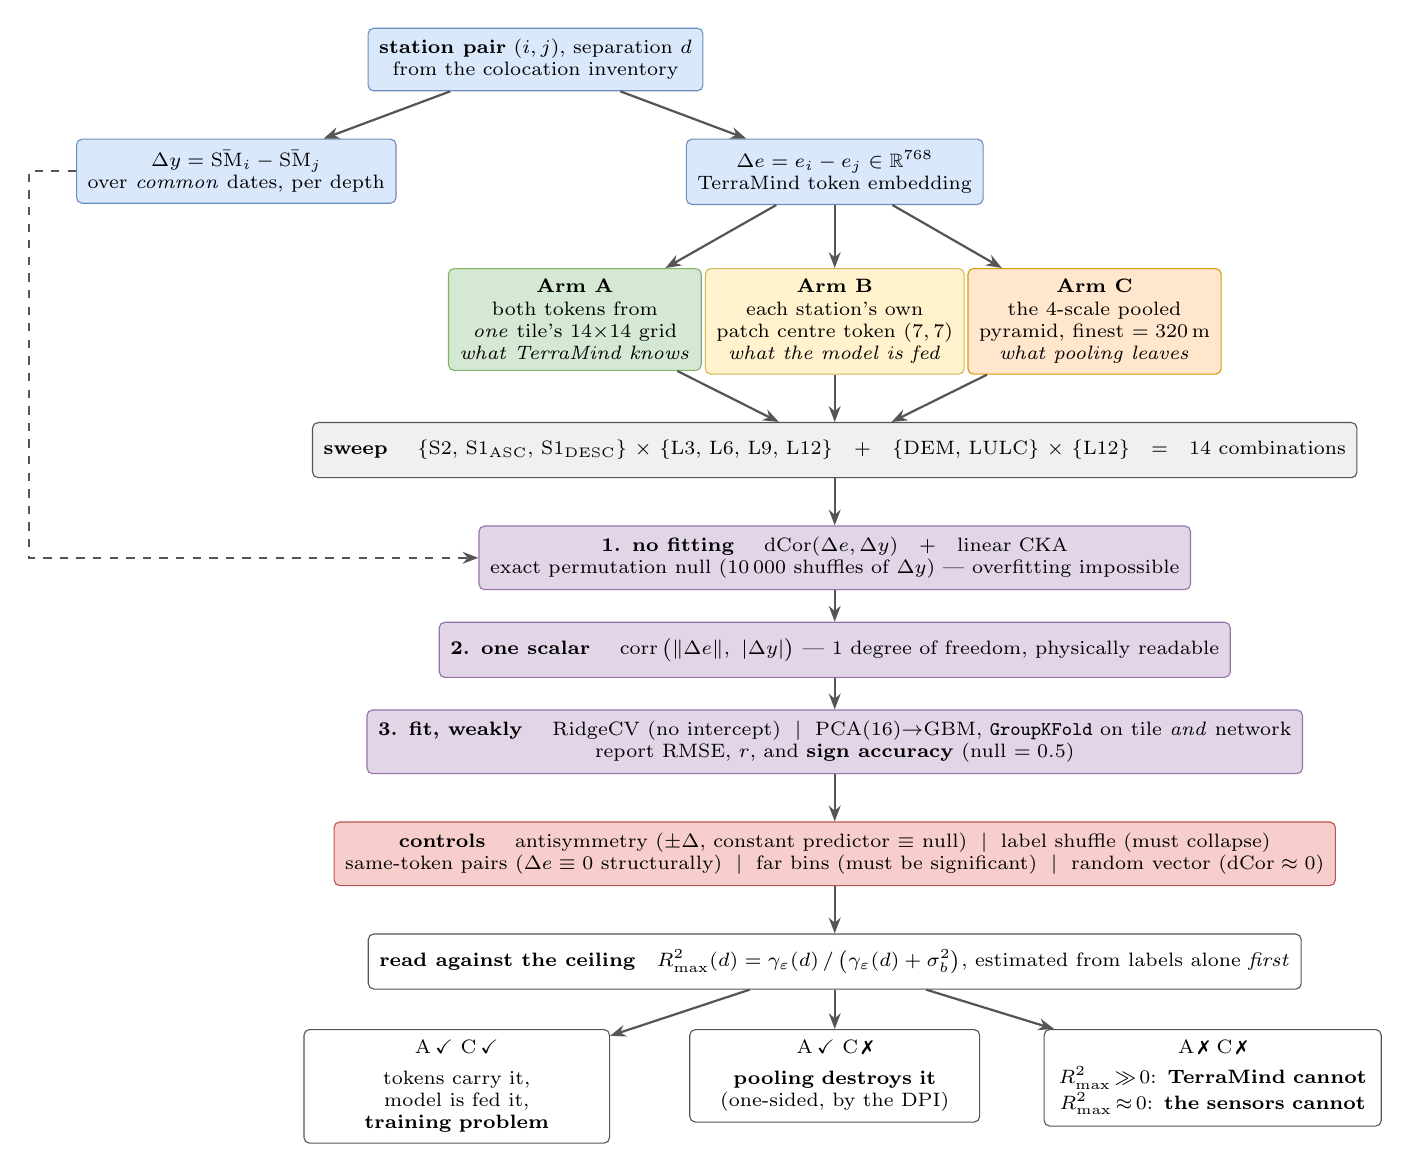
\begin{tikzpicture}[node distance=5mm]

\node[data] (pair) {\textbf{station pair} $(i,j)$, separation $d$\\
  from the colocation inventory};

\node[data, below=6mm of pair, xshift=-38mm] (dy)
  {$\Delta y = \bar{\mathrm{SM}}_i - \bar{\mathrm{SM}}_j$\\
   over \emph{common} dates, per depth};
\node[data, below=6mm of pair, xshift=38mm] (de)
  {$\Delta e = e_i - e_j \in \R^{768}$\\
   TerraMind token embedding};

\draw[ar] (pair) -- (dy);
\draw[ar] (pair) -- (de);

\node[armA, below=8mm of de, xshift=-33mm] (A)
  {\textbf{Arm A}\\ both tokens from\\ \emph{one} tile's 14$\times$14 grid\\
   \textit{what TerraMind knows}};
\node[armB, below=8mm of de] (B)
  {\textbf{Arm B}\\ each station's own\\ patch centre token $(7,7)$\\
   \textit{what the model is fed}};
\node[armC, below=8mm of de, xshift=33mm] (C)
  {\textbf{Arm C}\\ the 4-scale pooled\\ pyramid, finest $=320$\,m\\
   \textit{what pooling leaves}};

\draw[ar] (de) -- (A);
\draw[ar] (de) -- (B);
\draw[ar] (de) -- (C);

\node[box, below=6mm of B, fill=cGray] (sweep)
  {\textbf{sweep} \quad \{S2, S1$_{\text{ASC}}$, S1$_{\text{DESC}}$\} $\times$
   \{L3, L6, L9, L12\} \; + \; \{DEM, LULC\} $\times$ \{L12\} \; = \; 14 combinations};

\draw[ar] (A) -- (sweep);
\draw[ar] (B) -- (sweep);
\draw[ar] (C) -- (sweep);

\node[stat, below=6mm of sweep] (s1)
  {\textbf{1. no fitting} \quad $\dcor(\Delta e, \Delta y)$ \; + \; linear CKA\\
   exact permutation null (10\,000 shuffles of $\Delta y$) --- overfitting impossible};
\node[stat, below=4mm of s1] (s2)
  {\textbf{2. one scalar} \quad $\operatorname{corr}\big(\lVert\Delta e\rVert,\ |\Delta y|\big)$
   --- 1 degree of freedom, physically readable};
\node[stat, below=4mm of s2] (s3)
  {\textbf{3. fit, weakly} \quad RidgeCV (no intercept) $\;\vert\;$ PCA(16)$\to$GBM,
   \texttt{GroupKFold} on tile \emph{and} network\\
   report RMSE, $r$, and \textbf{sign accuracy} (null $=0.5$)};

\draw[ar] (sweep) -- (s1);
\draw[ar] (s1) -- (s2);
\draw[ar] (s2) -- (s3);

\node[ctrl, below=6mm of s3] (ctrl)
  {\textbf{controls} \quad
   antisymmetry ($\pm\Delta$, constant predictor $\equiv$ null) \;$\vert$\;
   label shuffle (must collapse) \\
   same-token pairs ($\Delta e \equiv 0$ structurally) \;$\vert$\;
   far bins (must be significant) \;$\vert$\;
   random vector ($\dcor \approx 0$)};

\draw[ar] (s3) -- (ctrl);

\node[verdict, below=6mm of ctrl] (gate)
  {\textbf{read against the ceiling} \;
   $R^2_{\max}(d) = \gamma_\varepsilon(d)\,/\,\big(\gamma_\varepsilon(d)+\sigma_b^2\big)$,
   estimated from labels alone \emph{first}};

\draw[ar] (ctrl) -- (gate);

\node[verdict, below=5mm of gate, xshift=-48mm, text width=36mm] (o1)
  {A\,\checkmark\ C\,\checkmark\\[1mm] tokens carry it, model is fed it,\\
   \textbf{training problem}};
\node[verdict, below=5mm of gate, xshift=0mm, text width=34mm] (o2)
  {A\,\checkmark\ C\,\ding{55}\\[1mm] \textbf{pooling destroys it}\\
   (one-sided, by the DPI)};
\node[verdict, below=5mm of gate, xshift=48mm, text width=40mm] (o3)
  {A\,\ding{55}\ C\,\ding{55}\\[1mm] $R^2_{\max}\!\gg\!0$: \textbf{TerraMind cannot}\\
   $R^2_{\max}\!\approx\!0$: \textbf{the sensors cannot}};

\draw[ar] (gate) -- (o1);
\draw[ar] (gate) -- (o2);
\draw[ar] (gate) -- (o3);

\draw[arf] (dy.west) -- ++(-6mm,0) |- (s1.west);

\end{tikzpicture}
\caption{The whole experiment. Blue = data, green/yellow/orange = the three embedding
arms, purple = the statistical ladder (least overfittable first), red = controls,
 and
white = interpretation.}
\label{fig:flow}
\end{figure}

\clearpage
\section{Mathematics}

\subsection{Model and estimand}

Let station $i$ sit at location $x_i$ and report a long-term mean
\begin{equation}
  y_i \;=\; \mu(x_i) \;+\; b_i,
  \qquad \E[b] = 0,\quad \Var(b) = \sigma_b^2,
  \label{eq:model}
\end{equation}
where $\mu(\cdot)$ is the true mean soil-moisture field and $b_i$ is a
\emph{station offset}: probe calibration, installation depth, local bulk density,
the mismatch between a point sensor and any areal quantity. Crucially $b_i$ is
\textbf{not} a property of the location --- two probes in the same soil pit would differ.

The embedding is $e_i = \varphi(x_i) \in \R^{768}$, the frozen TerraMind token covering
$x_i$. Decompose the field geostatistically,
\begin{equation}
  \mu(x) \;=\; m\big(z(x)\big) \;+\; \varepsilon(x),
  \label{eq:decomp}
\end{equation}
with $z$ the regional covariates (climate, biome, physiography) varying on a scale
$L \approx 100$\,km, and $\varepsilon$ a zero-mean short-range residual field with
variogram $\gamma_\varepsilon(d) = \tfrac12\E[(\varepsilon(x) - \varepsilon(x+d))^2]$.

We want to test whether $\varphi$ carries information about $\mu$ at short range:
\begin{equation}
  H_0:\quad \Delta e \;\perp\; \Delta \mu
  \quad\text{conditional on}\quad \lVert x_i - x_j\rVert = d,
  \qquad d \text{ small.}
\end{equation}

\subsection{Why the naive experiment fails, and differencing fixes it}

Regressing $y_i$ on $e_i$ across all 993 stations would succeed \emph{for the wrong
reason}: L12 encodes climate and biome, so it separates Texas from Norway. High $R^2$,
zero bearing on separating CR200-18 from CR200-6 at 936\,m.

Take differences instead. For a pair at separation $d \ll L$,
\begin{equation}
  \Delta\mu \;=\; \underbrace{\nabla m \cdot \Delta z}_{\to\, 0 \text{ as } d \to 0}
  \;+\; \Delta\varepsilon
  \;\;\longrightarrow\;\; \Delta\varepsilon .
  \label{eq:highpass}
\end{equation}
\textbf{The pair difference is a high-pass filter.} It annihilates everything varying on
scales $\gg d$ --- and it does so \emph{exactly}, not approximately, for anything constant
within the tile. Formally, for any nuisance variable $c$ the contribution to $\Delta y$ is
$c(x_i) - c(x_j)$, which is identically zero when $c$ is tile-constant. That covers:
climate, the ERA5-Land grid cell, rainfall history, season and date (we use common dates
only), biome, network operator, sensor vendor, calibration epoch --- and in Arm A, the
entire image context of the TerraMind forward pass, because both tokens come out of
\emph{one} forward pass on \emph{one} image.

Hence
\begin{equation}
  \Cov(\Delta e,\ \Delta y)
  \;=\; \underbrace{\Cov(\Delta e,\ \Delta\varepsilon)}_{\text{the quantity of interest}}
  \;+\; \underbrace{\Cov(\Delta e,\ \Delta b)}_{=\,0 \text{ in expectation}} .
  \label{eq:ident}
\end{equation}
The second term vanishes because sensor idiosyncrasy is not visible from orbit: $b$ is a
property of the instrument, independent of the land surface that $\varphi$ encodes.

\begin{quote}
\textbf{Identification claim.} A statistically significant association between $\Delta e$
and $\Delta y$ at small $d$ can only arise from genuine short-range field information in
the embedding. There is no confounder left to explain it away.
\end{quote}

This is the entire justification for the pair design, and it requires no modelling
assumption --- only that $b \perp \varphi$.

\subsection{The ceiling: what no method can beat}

From \eqref{eq:model},
\begin{equation}
  \Var(\Delta y) \;=\; 2\gamma_\varepsilon(d) \;+\; 2\sigma_b^2 ,
\end{equation}
so the maximum variance in $\Delta y$ that \emph{any} function of location can explain is
\begin{equation}
  \boxed{\;
  R^2_{\max}(d) \;=\; \frac{\gamma_\varepsilon(d)}{\gamma_\varepsilon(d) + \sigma_b^2}
  \;=\; \frac{\mathrm{SNR}(d)}{1 + \mathrm{SNR}(d)},
  \qquad \mathrm{SNR}(d) := \frac{\gamma_\varepsilon(d)}{\sigma_b^2}. \;}
  \label{eq:ceiling}
\end{equation}
As $d \to 0$, $\gamma_\varepsilon(d) \to 0$ while $\sigma_b^2$ does not. \textbf{Below some
separation, no covariate whatsoever can predict $\Delta y$}, because what remains is pure
instrument noise. This is a property of the observing system, not of the model.

$\sigma_b^2$ is estimable: it is the \textbf{nugget} of the empirical variogram
$\hat\gamma(d)$ of station-mean SM, read off by extrapolating $d \to 0$. For CR200-18,
$\hat\gamma(0.6\,\mathrm{km}) \approx 0.0601^2 = 0.0036$. If the nugget is of that same
order then $\mathrm{SNR} \approx 1$ and $R^2_{\max} \approx 0.5$: a probe scoring
$r \approx 0.5$ would be \emph{at the ceiling}, not failing.

\textbf{This must be computed before the embedding sweep is interpreted.} It costs minutes
and uses labels only. Reporting a null without it would be uninterpretable.

\subsection{The test statistic, and why it is legitimate at $n \ll p$}

For random vectors $U \in \R^{p}$, $V \in \R^{q}$ with finite first moments, the distance
correlation of Sz\'ekely, Rizzo and Bakirov satisfies
\begin{equation}
  \dcor(U,V) = 0 \quad\Longleftrightarrow\quad U \perp V .
\end{equation}
Unlike Pearson correlation it detects \emph{any} dependence, linear or not, and unlike
mutual information it is estimable at small $n$. It has \textbf{no fitted parameters}, so
overfitting is structurally impossible, and under $H_0$ the labels $\Delta y$ are
exchangeable, making the permutation null \textbf{exact} rather than asymptotic.
With $B = 10^4$ permutations the $p$-value $(1 + \#\{\dcor^\ast \ge \dcor\})/(1+B)$ is
valid for any $n$ and any $p$.

\paragraph{The one real hazard: distance concentration.} In high dimension, pairwise
Euclidean distances concentrate,
$\Var(\lVert \Delta e\rVert)/\E[\lVert \Delta e\rVert]^2 \to 0$ as $p \to \infty$, which
attenuates $\dcor$ towards zero and costs power (it does not create false positives ---
the test stays valid, just conservative). Two mitigations, both leakage-free:
\begin{enumerate}[nosep]
  \item standardise each of the 768 coordinates using statistics computed on
        \emph{far} pairs only;
  \item project $\Delta e$ onto the leading $k \approx 16$ principal components of the
        \emph{far}-pair difference matrix. Far pairs never enter the near-pair test, so
        no information leaks across the hypothesis being tested.
\end{enumerate}

\subsection{The resolution curve, and its built-in positive control}

Define, per separation bin,
\begin{equation}
  \rho(d) \;:=\; \dcor\big(\Delta e,\ \Delta y \;\big|\; \lVert x_i - x_j \rVert \in d\big).
\end{equation}
We already know $\rho$ must be large at continental range: between-network level
correlation is $r = +0.85$ (Table~\ref{tab:scale}). Therefore
\textbf{the far bins are the positive control}, computed with the identical statistic on
the identical pipeline. No separately-constructed control is needed, and a pipeline bug
that kills the signal would be caught where we \emph{know} signal exists.

The separation at which $\rho(d)$ becomes indistinguishable from its permutation null is
then a definition, not an inference: it \textbf{is} the effective level resolution of the
embedding.

\subsection{Arm A versus Arm C is a data-processing inequality}

Pooling is a fixed, data-independent map $P$ (\verb|_cpu_pyramid_pool|,
\verb|dataset.py:190-220|) applied to the token grid. By the data-processing inequality,
for any target $y$,
\begin{equation}
  I\big(P\!\cdot\!e \,;\, y\big) \;\le\; I\big(e \,;\, y\big)
  \qquad\Longrightarrow\qquad \rho_C \;\le\; \rho_A \ \ \text{in expectation.}
\end{equation}
The comparison is therefore \textbf{one-sided by construction} --- pooling can only
destroy information, never create it. If $\rho_A > 0$ while $\rho_C \approx 0$, we have
not merely observed a correlation: we have \emph{proved} that the bottleneck is our
pooling operator, not TerraMind.

\subsection{Antisymmetry is a free guarantee}

The labelling of $i$ versus $j$ is arbitrary, so the joint law of $(\Delta e, \Delta y)$ is
invariant under $(\Delta e, \Delta y) \mapsto (-\Delta e, -\Delta y)$. Emitting both
orderings of every pair makes this exact in the sample. Three consequences:
\begin{enumerate}[nosep]
  \item $\E[\Delta y] = \E[\Delta e] = 0$ \emph{exactly}; the intercept is zero and must be
        fitted as zero (\verb|fit_intercept=False|).
  \item Any constant predictor achieves \emph{exactly} the null RMSE. There is no free
        lunch from predicting the mean --- the failure mode that makes ordinary
        station-level regression look better than it is.
  \item The true regression function is odd, $f(-\Delta e) = -f(\Delta e)$. Ridge without
        intercept satisfies this automatically; the GBM is symmetrised by the augmentation.
\end{enumerate}

\subsection{Same-token pairs are an exact structural zero}

A token covers $16 \times 16$ px $= 160$\,m. Two stations closer than 160\,m
(and not straddling a token boundary) fall in the \emph{same} token, so in Arm A
\begin{equation}
  \Delta e \;\equiv\; 0 \qquad\text{exactly, by construction,}
\end{equation}
while $\Delta y \ne 0$ in general. These pairs are simultaneously:
\begin{itemize}[nosep]
  \item a \textbf{perfect negative control} --- any nonzero apparent skill on them is a bug;
  \item a \textbf{direct estimate of the floor}: $\Var(\Delta y \mid \text{same token})
        = 2\gamma_\varepsilon(d_{<160\mathrm{m}}) + 2\sigma_b^2$, which bounds
        $\sigma_b^2$ from above without any variogram extrapolation.
\end{itemize}
Per \S26.10 this is not a hypothetical: of 95 temporally-usable in-tile pairs, roughly
62 are sub-token. They are not wasted --- they measure the ceiling.

\clearpage
\section{Design}

\subsection{Unit of analysis}

For two stations $i,j$ inside the same tile, per depth,
\[
  \Delta y_{ij} = \bar{\mathrm{SM}}_i - \bar{\mathrm{SM}}_j
  \quad\text{over their \emph{common} observed dates (QC-clean only)},
  \qquad
  \Delta e_{ij} = e_i - e_j .
\]
Requiring common dates matters: differing record windows would reintroduce climate through
the back door (a station observed only in a drought year is drier for reasons unrelated to
place). \S26.10 found temporal overlap, not geometry, is the binding constraint.

Station at pixel $(r,c)$ lands in token $(\lfloor r/16\rfloor, \lfloor c/16\rfloor)$.
The CR200-18 figure lists all six token indices --- 105, 62, 100, 20, 44, 172 --- so for
that tile all six embeddings are genuinely distinct vectors.

\subsection{The three arms}

\begin{table}[h]
\centering\small
\begin{tabular}{@{}p{12mm}p{58mm}p{72mm}@{}}
\toprule
arm & embedding taken from & question it answers \\
\midrule
\textbf{A} & both stations read from \emph{one} tile's 14$\times$14 grid at their own token
             indices
           & does TerraMind's representation distinguish two points 160--900\,m apart
             \emph{within one image}? \\[1mm]
\textbf{B} & each station uses the centre token $(7,7)$ of its \emph{own} patch
           & is the finest thing the model is actually fed discriminative? \\[1mm]
\textbf{C} & the 4-scale pooled pyramid the model really receives
             (\texttt{dataset.py:190-220})
           & does the pooling destroy it? \\
\bottomrule
\end{tabular}
\caption{Arm A is what TerraMind knows; Arm C is what the model is told. The gap between
them is our engineering, not TerraMind's limit.}
\end{table}

Arm B additionally unlocks \emph{all} pairs at \emph{any} separation --- stations need not
share a tile --- which is what makes the $\rho(d)$ curve of \S4.5 estimable with large $n$.

\subsection{Layer $\times$ modality sweep}

Verified on \verb|ISMN_TxSON_CR200-18| (read-only, 2026-08-12):

\begin{table}[h]
\centering\small
\begin{tabular}{@{}lll@{}}
\toprule
modality & arrays present & shape \\
\midrule
\verb|s2/{l3,l6,l9,l12}|                    & all four layers & \verb|(178, 196, 768)| fp16 \\
\verb|s1_asc/…|, \verb|s1_desc/…|           & all four layers & \verb|(184, 196, 768)| fp16 \\
\verb|dem|, \verb|lulc|                     & \textbf{L12 only} & \verb|(196, 768)| fp16 \\
\bottomrule
\end{tabular}
\end{table}

Sweep $=$ \{S2, S1$_{\text{ASC}}$, S1$_{\text{DESC}}\} \times \{$L3, L6, L9, L12$\}$ $+$
\{DEM, LULC\} $\times$ \{L12\} $=$ \textbf{14 combinations} $\times$ 3 arms.

\paragraph{The hypothesis this sweep tests.} L12 is semantic --- it is where site identity
lives, which \S24.12 showed dominates the model's behaviour. L3 and L6 are shallower and
closer to raw radiometry, which is where a 160\,m wetness contrast would live if it lives
anywhere. \textbf{We predict early layers beat L12 on within-tile contrast even though
L12 beats them on site identity.} A layer-monotone result either way is a real finding
about what foundation-model features are for.

Temporal aggregation matches the target: $\Delta y$ is a multi-year mean, so the primary
feature is the multi-year mean token. Seasonal means and the temporal SD of the token
enter as secondary blocks.

DEM and LULC at L3/L6/L9 do not exist and would require a GPU re-run of
\verb|precompute_terramind.py| (one static forward per station, no time axis). Gated:
do not pay for it unless the S2/S1 sweep shows early layers matter.

\subsection{Statistical ladder and controls}

Ordered least-overfittable first, per Figure~\ref{fig:flow}. Controls:

\begin{description}[nosep,leftmargin=1.6em]
  \item[Antisymmetry] both orderings emitted; a constant predictor sits exactly at the null.
  \item[Label shuffle] permute $\Delta y$ within folds; every combination must collapse.
        Mandatory at $p=768$, $n\sim 33$.
  \item[Same-token pairs] $\Delta e \equiv 0$; any apparent skill is a bug (\S4.8).
  \item[Far bins] must be significant --- the built-in positive control (\S4.5).
  \item[Random vector] a random $\R^{768}$ vector per station must give $\dcor \approx 0$.
  \item[Independent positive control] the same machinery on $\Delta$(elevation) and
        $\Delta$(soil texture) at the station pixel, which demonstrably vary in this tile
        (450.8--467.9\,m; SOC 161--175). If nothing is detected there either, the machinery
        is broken, not TerraMind. This is the analogue of \S24's ERA5-shuffle control,
        which is what made \S24 interpretable.
\end{description}

\section{Data inventory}
\label{sec:inventory}

\subsection{Pair counts --- and the honest number}

Great-circle sweep over all 993 stations in \verb|csvs/station_splits.csv|
(computed 2026-08-12):

\begin{table}[h]
\centering\small
\begin{tabular}{@{}lr@{\qquad}lr@{}}
\toprule
separation & pairs & separation & pairs \\
\midrule
$<0.5$\,km      & 46  & 2.24--5\,km   & 178 \\
0.5--1\,km      & 23  & 5--10\,km     & 283 \\
1--2.24\,km     & 57  & 10--30\,km    & 1\,420 \\
\textbf{$<2.24$\,km total} & \textbf{126} & 30--100\,km & 4\,287 \\
                &     & $>100$\,km    & 486\,234 \\
\bottomrule
\end{tabular}
\end{table}

The 126 span \textbf{12 networks} --- TxSON 55, FMI 22, SNOTEL 13, AmeriFlux 11, SCAN 5,
ICOS 4, ARM 3, FLUXNET-AMERIFLUX 3, SOILSCAPE 3, iRON 2, Berlin 1, NGARI 1 --- so Arm A is
not confined to one catchment or one climate.

\paragraph{But geometry is not the binding constraint.} \S26.10 already ran this inventory
properly, including the 482 level-1 stations outside the pipeline, and found:
33 colocation clusters covering 105 stations; 206 ordered in-tile pairs; \textbf{95 usable
at $\ge 365$\,d record overlap}; and restricting to $\ge 160$\,m separation --- required
for $\Delta e \ne 0$ in Arm A --- leaves \textbf{33 unique pairs}. Sixty-four in-tile pairs
are lost purely to non-overlapping records, including the 7-node SOILSCAPE deployment
inside Tonzi Ranch's tile.

\begin{quote}
\textbf{So Arm A's real sample size is $n \approx 33$ (66 with both orderings), not 126.}
This is the single most important number in this document and it must be stated in any
write-up. It is why the ladder begins with a parameter-free statistic and an exact
permutation test, and why Arm B and the $\rho(d)$ curve --- where $n$ is in the thousands
--- carry the statistical weight.
\end{quote}

\subsection{Depth}

0--10\,cm is primary: it is where satellite sensing has physical justification and where
the tile figure fails. 10--30 and 30--100 are reported as secondary. Note TxSON is
\textbf{surface-only} (\S26.2), so the deeper analysis draws on the non-TxSON clusters.
\S24.12 found deep prediction is close to a pure site fingerprint (temporal share only
12\,\% at 30--100), so the depth dependence is itself informative.

\subsection{Multiplicity}

14 (modality $\times$ layer) $\times$ 3 arms $\times$ 3 depths $\times$ 8 distance bins.
\textbf{Pre-registered primary test: depth 0--10, Arm A, S2, all bins.} Everything else is
exploratory and reported under Benjamini--Hochberg FDR. The gate is \emph{not} a
max-over-tests.

\section{How each outcome is read}

Always jointly with the ceiling $R^2_{\max}(d)$ of \S4.3 --- a probe that reaches the
ceiling has succeeded even if its absolute $r$ looks modest.

\begin{table}[h]
\centering\small
\begin{tabular}{@{}llp{52mm}p{52mm}@{}}
\toprule
Arm A & Arm C & conclusion & next move \\
\midrule
signal & signal & tokens carry it, the model is fed it, the model fails to use it
       & training/loss problem: multi-station supervision, level/anomaly decomposition \\[1mm]
signal & none   & \textbf{pooling destroys it} --- guaranteed one-sided by the DPI
       & cheapest fix in the project: restore a true 1$\times$1 centre scale, exempt the
         centre token from the 50\,\% dropout \\[1mm]
none   & none, $R^2_{\max}\!\gg\!0$ & TerraMind at 160\,m does not resolve sub-km SM contrast
       & state the resolution limit; reframe on ubRMSE / NSE$_{\text{anom}}$ \\[1mm]
none   & none, $R^2_{\max}\!\approx\!0$ & the \emph{observations} cannot resolve it ---
         station offset noise exceeds the true field contrast
       & not a model finding at all; report the nugget and stop \\
\bottomrule
\end{tabular}
\end{table}

Valid only if $\rho(d)$ is significant in the far bins and the random-vector control gives
$\dcor \approx 0$.

\section{Limitations, stated up front}

\begin{enumerate}[nosep]
  \item \textbf{$n \approx 33$ for Arm A.} A null is weak evidence of absence and must be
        reported as underpowered, never as ``TerraMind cannot''. Power, not validity, is
        the constraint --- the permutation test is exact at any $n$.
  \item \textbf{$\Delta b$ is irreducible.} Part of every observed contrast is instrument,
        not landscape. \eqref{eq:ceiling} quantifies how much; it cannot be removed.
  \item \textbf{A 160\,m token cannot be expected to resolve a point sensor.} ISMN probes
        integrate over centimetres. Even a perfect 160\,m representation predicts the
        160\,m areal mean, not the probe. This is a fundamental support mismatch and it
        contributes to $\sigma_b^2$.
  \item \textbf{Arm A tests the representation, not the model.} A positive Arm A does not
        imply the current architecture could exploit it; that is what Arm C and the
        deferred multi-station-supervision work would establish.
  \item \textbf{Colocated stations are geographically clustered.} Even across 12 networks,
        clusters are not a random sample of the Earth. Conclusions generalise to
        ``dense-network conditions'', not globally.
  \item \textbf{Mean SM is one summary.} Two stations could share a mean and differ in
        dynamic range. This experiment deliberately targets level, because level is where
        the model fails (bias$^2 \approx 50\,\%$ of MSE per \S22.10).
\end{enumerate}

\section{What gets built, after this document is approved}

\begin{itemize}[nosep]
  \item \verb|build_network_readouts.py| --- add \verb|--all-networks|, writing
        \verb|csvs/all_readouts.csv|; reuse the existing centre assertion (\verb|:214|) and
        forward/reverse offset symmetry check (\verb|:230|). Must reproduce
        \verb|csvs/txson_readouts.csv| when filtered to TxSON.
  \item \verb|probe_variogram.py| --- \S4.3, labels only, minutes. Produces $\hat\gamma(d)$,
        the nugget, and $R^2_{\max}(d)$ per depth. \textbf{Runs first.}
  \item \verb|probe_terramind_subkm.py| --- the sweep. Modelled on
        \verb|station_mean_probe.py|: CPU-only, \verb|Pool(64)|, opens zarr per station
        directly (never instantiates \verb|SoilMoistureDataset|, which eagerly loads
        $\sim$16\,GB of L12 tokens). Reuses \verb|_load_zarr_labels| and
        \verb|_cpu_pyramid_pool| from \verb|dataset.py|.
  \item \verb|slurm/probe_terramind_subkm.sh| --- CPU partition,
        \verb|--cpus-per-task=64|, \verb|--mail-type=BEGIN,END,FAIL|,
        \verb|--mail-user=ktm.prajwalkhanal@gmail.com|. Nothing runs interactively.
  \item Outputs: \verb|csvs/subkm_pairs.csv|, \verb|csvs/terramind_subkm_probe.json|,
        \verb|figures/subkm_layer_sweep.png| (dCor heat-map, layer $\times$ modality
        $\times$ arm), \verb|figures/subkm_rho_curve.png| (the $\rho(d)$ resolution curve).
\end{itemize}

\paragraph{Verification before any number is trusted.}
(i) every station projects into its own tile at exactly $(112,112)$;
(ii) the six CR200-18 station means reproduce the figure's values
$(0.1367, 0.1197, 0.1826, 0.2323, 0.1857, 0.2865)$ to $10^{-3}$;
(iii) for a tile's centre station, its Arm A token and Arm B token are bit-identical;
(iv) $\lVert\Delta e\rVert = 0$ exactly on same-token pairs;
(v) $\sum \Delta y = 0$ exactly over the antisymmetrised table;
(vi) all 14 combinations collapse to the null under permuted labels.

\end{document}
